\documentclass[border=3mm]{standalone}

\usepackage{tikz}
\usetikzlibrary{decorations.markings}

\begin{document}
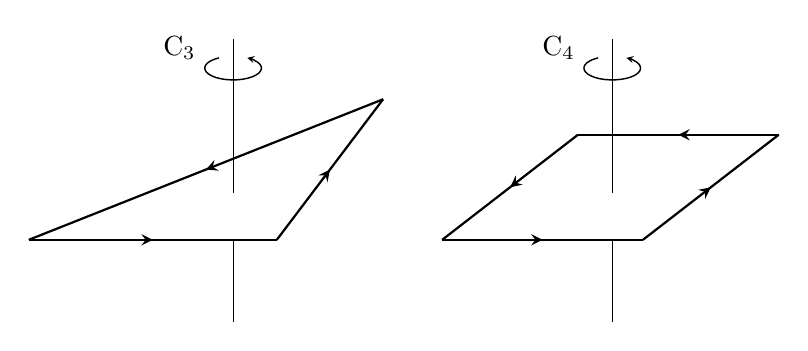
\begin{tikzpicture}[scale=0.75]
\newcommand{\AxisRotator}[1][rotate=0]{%
    \tikz [x=0.25cm,y=0.60cm,line width=.2ex,-stealth,#1] \draw (0,0) arc (-150:150:1 and 1);%
}
\draw (-2.94,-3) -- (-2.94,-0.8);
\begin{scope}[very thick,decoration={
    markings,
    mark=at position 0.5 with {\arrow{stealth}}}
    ]
\fill[white] (-6.4,-1.6) -- (-2.2,-1.6) -- (-0.4,0.78) -- cycle;
\draw[thick,postaction={decorate}] (-6.4,-1.6) -- (-2.2,-1.6);
\draw[thick,postaction={decorate}] (-2.2,-1.6) -- (-0.4,0.78);
\draw[thick,postaction={decorate}] (-0.4,0.78) -- (-6.4,-1.6);
\end{scope}
\draw (-2.94,-0.8) -- (-2.94,1.8) node[pos=0.8,rotate=-90,scale=0.6] {\AxisRotator} node[pos=0.8,above left,xshift=-10pt]{C\textsubscript{3}};

\draw (3.48,-3) -- (3.48,-0.8);
\begin{scope}[very thick,decoration={
    markings,
    mark=at position 0.5 with {\arrow{stealth}}}
    ]
\fill[white] (0.6,-1.6) -- (4,-1.6) -- (6.3,0.18) -- (2.9,0.18) -- cycle;
\draw[thick,postaction={decorate}] (0.6,-1.6) -- (4,-1.6);
\draw[thick,postaction={decorate}] (4,-1.6) -- (6.3,0.18);
\draw[thick,postaction={decorate}] (6.3,0.18) -- (2.9,0.18);
\draw[thick,postaction={decorate}] (2.9,0.18) -- (0.6,-1.6);
\end{scope}
\draw (3.48,-0.8) -- (3.48,1.8) node[pos=0.8,rotate=-90,scale=0.6] {\AxisRotator} node[pos=0.8,above left,xshift=-10pt]{C\textsubscript{4}};
\end{tikzpicture}
\end{document}